% Single-file Quantum manuscript draft. No \input, no external .bib required.
\documentclass[a4paper,onecolumn,11pt]{quantumarticle}
\pdfoutput=1
\usepackage[english]{babel}
\usepackage[T1]{fontenc}
\usepackage[utf8]{inputenc}
\usepackage{amsmath,amssymb,bm,mathtools}
\usepackage{physics}
\usepackage{booktabs}
\usepackage{csquotes}
\usepackage{enumitem}
\usepackage{xcolor}
\usepackage{tikz}
\usetikzlibrary{arrows.meta,positioning,calc,decorations.pathreplacing,shapes.geometric}
\usepackage{hyperref}
\hypersetup{colorlinks=true,linkcolor=blue!50!black,citecolor=blue!50!black,urlcolor=blue!50!black}

% Shorthands
\newcommand{\ii}{\ensuremath{\mathrm{i}}}
\newcommand{\bbI}{\ensuremath{\mathbb{I}}}
\newcommand{\bbR}{\ensuremath{\mathbb{R}}}
\newcommand{\bbC}{\ensuremath{\mathbb{C}}}
\def\vk{\ensuremath{\bm{k}}}
\def\vq{\ensuremath{\bm{q}}}
\def\vp{\ensuremath{\bm{p}}}
\def\vsigma{\ensuremath{\bm{\sigma}}}
\def\vtau{\ensuremath{\bm{\tau}}}
\def\vdelta{\ensuremath{\bm{\delta}}}
\newcommand{\Hop}{\ensuremath{H}}
\newcommand{\Uop}{\ensuremath{U}}
\newcommand{\UW}{\ensuremath{U_{W}}}
\newcommand{\UD}{\ensuremath{U_{D}}}
\newcommand{\HD}{\ensuremath{H_{D}}}
\newcommand{\HW}{\ensuremath{H_{W}}}
\newcommand{\Lattice}{\ensuremath{\Lambda}}
\newcommand{\Proto}{\ensuremath{\mathfrak{P}_{\mathrm{disc}}}}
\newcommand{\gmu}{\ensuremath{\gamma^{\mu}}}
\newcommand{\gnu}{\ensuremath{\gamma^{\nu}}}
\newcommand{\sigmunu}{\ensuremath{\Sigma^{\mu\nu}}}

\title{Emergent Dirac dynamics from discrete quantum walks: a verified infrared construction}

\author{Nelson Bol\'ivar}
\affiliation{Astrum Drive Technologies, astrumdrivetechnologies@gmail.com}
\date{May 11, 2026}

\begin{document}
\maketitle

\begin{abstract}
We present a compact construction of emergent Dirac dynamics from local discrete quantum walks. The central point is a separation of levels: microscopic locality and exact discrete symmetries at Level I, infrared Weyl/Dirac dynamics at Level II, and covariant spinorial organization at Level III. Starting from SSH and graphene as calibration examples, we isolate the algebraic mechanism by which a honeycomb quantum walk yields a $2{+}1$-dimensional Dirac Hamiltonian, then extend the ladder to Weyl nodes, four-component Dirac sectors, controlled Weyl splitting, and Wilson-type control of doublers in three dimensions. We finally reconstruct the covariant data of the continuum theory, including the Clifford algebra, spinorial Lorentz generators, and the $SL(2,\bbC)$ double-cover structure. A distinctive feature of the construction is methodological: the algebraic identities supporting the infrared limit are paired with lightweight symbolic checks in \texttt{sympy} and \texttt{z3}. The result is not a microscopic derivation of exact Lorentz invariance, but a verified infrared construction that makes precise which Dirac-covariant structures can emerge from local discrete dynamics, and which structural questions remain open beyond reciprocal-space periodicity.
\end{abstract}


\section{Introduction}
\label{p:intro}

The $(3+1)$-dimensional Dirac equation, the Clifford algebra it sits on, and the spinorial Lorentz generators that organize it are usually introduced in the continuum, where smooth spacetime and continuous symmetry groups are already available. A persistent question, going back to Wilson's lattice fermions and sharpened by the Nielsen--Ninomiya obstruction~\cite{Wilson1974,NielsenNinomiya1981a,NielsenNinomiya1981b}, is how much of this relativistic structure can instead be recovered as an infrared sector of a local discrete dynamics. Quantum walks and quantum cellular automata provide a natural modern arena for this question~\cite{Arrighi2018,FarrellyShort2014,Farrelly2020}.

This paper does not claim that Lorentz covariance is exact microscopically. The aim is narrower and more auditable: to identify which algebraic data of Dirac covariance are recovered in the infrared sector of local discrete dynamics, and to pair the identities supporting that recovery with machine-checkable symbolic tests.

% Figure 1: dimensional ladder
\begin{figure*}[t]
\centering
\resizebox{\textwidth}{!}{%
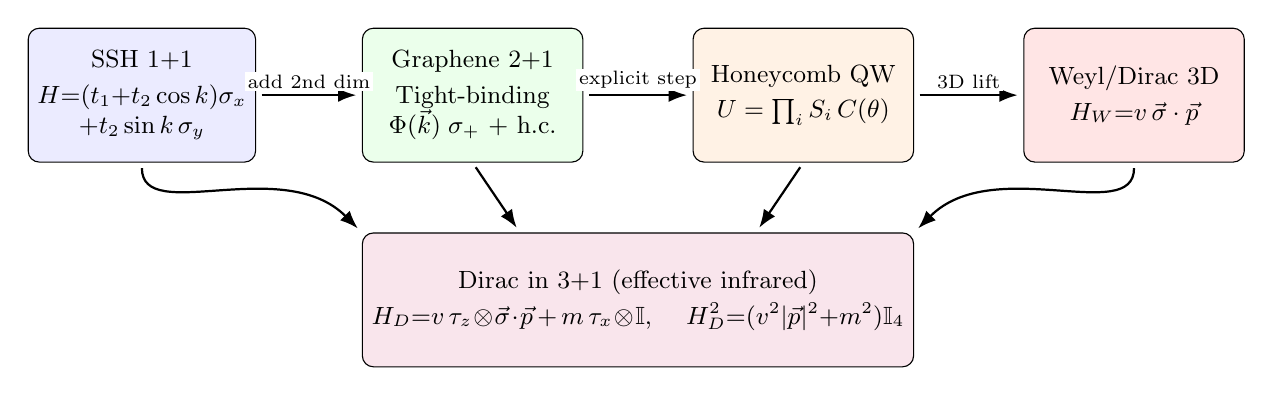
\begin{tikzpicture}[
  every node/.style={align=center, font=\small},
  box/.style={draw, rounded corners, minimum width=2.8cm, minimum height=1.7cm,
              align=center, font=\small},
  arr/.style={->, >=Latex, thick, shorten >=2pt, shorten <=2pt},
]
  % Top row: discrete models
  \node[box, fill=blue!8]   (ssh)  at (0,2)
    {SSH 1+1\\[2pt]\(H{=}(t_1{+}t_2\cos k)\sigma_x\)\\\(+ t_2\sin k\,\sigma_y\)};
  \node[box, fill=green!8]  (gr)   at (4.2,2)
    {Graphene 2+1\\[2pt]Tight-binding\\\(\Phi(\vec k)\;\sigma_+\) {+} h.c.};
  \node[box, fill=orange!10] (qw)  at (8.4,2)
    {Honeycomb QW\\[2pt]\(U=\prod_i S_i\,C(\theta)\)};
  \node[box, fill=red!10]   (wd)   at (12.6,2)
    {Weyl/Dirac 3D\\[2pt]\(H_W{=}v\,\vec\sigma\cdot\vec p\)};

  % Bottom: continuum target
  \node[box, fill=purple!10, minimum width=5cm] (dirac) at (6.3,-0.6)
    {Dirac in 3+1 (effective infrared)\\[2pt]
     \(H_D{=}v\,\tau_z\!\otimes\!\vec\sigma\!\cdot\!\vec p \,{+}\, m\,\tau_x\!\otimes\!\bbI\),
     \quad \(H_D^2{=}(v^2|\vec p|^2{+}m^2)\bbI_4\)};

  % Arrows along the top row
  \draw[arr] (ssh) -- node[above, font=\scriptsize, fill=white, inner sep=1pt, yshift=1pt]
              {add 2nd dim} (gr);
  \draw[arr] (gr) -- node[above, font=\scriptsize, fill=white, inner sep=1pt, yshift=1pt]
              {explicit step} (qw);
  \draw[arr] (qw) -- node[above, font=\scriptsize, fill=white, inner sep=1pt, yshift=1pt]
              {3D lift} (wd);

  % Arrows from each top box down to Dirac 3+1
  \draw[arr] (ssh.south) .. controls +(0,-0.8) and +(-1,1) .. (dirac.north west);
  \draw[arr] (gr.south) -- ([xshift=-1.5cm]dirac.north);
  \draw[arr] (qw.south) -- ([xshift=1.5cm]dirac.north);
  \draw[arr] (wd.south) .. controls +(0,-0.8) and +(1,1) .. (dirac.north east);

  % Side label
  \node[font=\footnotesize\itshape, right=0.2cm of wd, xshift=-0.3cm, yshift=-0.4cm] {};
\end{tikzpicture}
}%
\caption{The dimensional ladder. Four discrete models (top row) all flow
under linearization plus continuum limit to the same effective Dirac block
in $3{+}1$ (bottom). The algebraic objects that survive the limit
(Clifford algebra, $\Sigma^{\mu\nu}$, chirality balance) are the same at
each rung.}
\label{p:fig:ladder}
\end{figure*}


\subsection*{Contributions}

\paragraph{1.~Level separation.}
We separate three logically distinct layers: Level I contains the microscopic step and its exact locality/symmetry data; Level II contains the infrared Weyl/Dirac Hamiltonians obtained by linearization; Level III contains the covariant spinorial organization by Clifford generators, Lorentz generators, and the $SL(2,\bbC)$ double cover. This separation is the guardrail against over-reading effective Lorentz covariance as a microscopic symmetry.

\paragraph{2.~A verified Dirac ladder.}
We assemble a single coherent ladder,
\[
\text{SSH in }1{+}1 \;\longrightarrow\;
\text{graphene in }2{+}1 \;\longrightarrow\;
\text{honeycomb QW} \;\longrightarrow\;
\text{Weyl/Dirac in }3{+}1,
\]
with uniform notation throughout. SSH and graphene are used as calibration examples rather than as novel claims; the honeycomb walk makes the discrete-to-continuum transition explicit; and the 3D construction exhibits Weyl chirality, Dirac doubling, controlled Weyl splitting, and Wilson-type control of the extra lattice sectors.

\paragraph{3.~Verification as build discipline.}
The construction is accompanied by a lightweight verification pipeline. \texttt{sympy} checks closed-form matrix identities, Taylor expansions, Clifford anticommutators, Lorentz-generator commutators, and dispersion relations. \texttt{z3}~\cite{deMoura2008} checks finite combinatorial constraints such as chirality balance, isotropy consistency, and graph-based structural statements. The goal is not to replace formal proof assistants, but to make the algebraic layer of the manuscript locally auditable.

\paragraph{Scope.}
The construction is not unique, and it does not determine a final microscopic substrate. Its role is to establish a verified infrared ladder and to isolate the next structural problem: formulating locality, chirality, and Dirac sectors without assuming reciprocal-space periodicity from the start.


\section{Setup, notation, and three levels}
\label{p:setup}

\subsection{Notation}
We use the following conventions.
$\vk$ denotes a Bloch momentum on the discrete model, $\vq$ a small
deviation about a band-crossing point $\vk_{0}$, and $\vp$ the continuum
infrared momentum. Internal degrees of freedom are organized by
$\sigma_{i}$ (pseudospin / Weyl two-component) and $\tau_{i}$ (chiral
index or coupled-block label). The canonical four-component Dirac block
that we recover at the end of the ladder takes the form
\begin{equation}
\HD \;=\; v\,\tau_{z} \otimes (\sigma_{x} p_{x} + \sigma_{y} p_{y} + \sigma_{z} p_{z})
            \;+\; m\,\tau_{x}\otimes\bbI ,
\label{p:eq:HDcanon}
\end{equation}
whose squared form
$\HD^{2} = (v^{2}\lvert \vp\rvert^{2} + m^{2})\,\bbI_{4}$
will reappear several times.

\subsection{Three levels}
A recurring source of confusion in this corner of the literature is the
conflation of three distinct levels of statement. We commit to keeping
them apart throughout the paper:

\begin{description}
\item[\textbf{Level I (microscopic exact).}]
    The discrete substrate: lattice or step protocol $\Uop$, locality, the
    exact group of discrete symmetries, quasi-energy periodicity in
    discrete-time models. At this level the fundamental dynamical object
    is $\Uop$, not $\Hop$.
\item[\textbf{Level II (effective infrared).}]
    The linearization around a band-crossing point, the appearance of
    Weyl or Dirac blocks, approximate continuous isotropy, the reading
    of mass, chirality, and effective velocity. Here it is natural to
    write $\Uop \simeq \bbI - \ii\,\Delta t\,\Hop_{\mathrm{eff}}$.
\item[\textbf{Level III (covariant spinorial).}]
    The Clifford algebra of $\gmu$, the spinorial Lorentz generators
    $\sigmunu$, the proper orthochronous group $SO^{+}(3,1)$,
    Poincar\'e, and the double-cover $SL(2,\bbC) \to SO^{+}(3,1)$. This
    level is the \emph{organization} of the infrared limit, not an exact
    symmetry of the substrate.
\end{description}

We will reserve the adjective \enquote{exact} for Level I, and the
adjective \enquote{effective} or \enquote{infrared} for Levels II and
III. This split, banal as it sounds, is what saves the rest of the
construction from over-claiming.

\subsection{The protospace tuple}
By \emph{protospace} we mean the ampliated structure that carries the
microscopic dynamics:
\begin{equation}
\Proto \;\sim\; \bigl(\Lattice,\,\bbC^{N},\,\Uop,\,G_{\mathrm{micro}}\bigr) ,
\label{p:eq:proto-tuple}
\end{equation}
where $\Lattice$ is the underlying graph (not necessarily periodic),
$\bbC^{N}$ the local internal Hilbert space, $\Uop$ the local step, and
$G_{\mathrm{micro}}$ its exact discrete symmetry group. Identifying
$\Proto$ with the Brillouin torus $T^{d}$ would confuse a
\emph{calculational device} (the Fourier-space representation of a
periodic protocol) with the \emph{underlying structure}. We come back to
this point in Section~\ref{p:open-problems}.


\section{SSH \texorpdfstring{$\rightarrow$}{->} Dirac in \texorpdfstring{$1{+}1$}{(1+1)}}
\label{p:ssh}

The first rung of the ladder is the Su--Schrieffer--Heeger model~\cite{Su1979} on a
1D chain with two sites per unit cell and bond alternation $(t_1, t_2)$.
The Bloch Hamiltonian in the standard convention is
\begin{equation}
\Hop_{\mathrm{SSH}}(k)
    = (t_1 + t_2 \cos k)\,\sigma_x + t_2\,\sin k\,\sigma_y ,
\label{p:eq:HSSH}
\end{equation}
with dispersion
$E_{\pm}(k) = \pm\sqrt{t_1^2 + 2 t_1 t_2 \cos k + t_2^2}$.
The gap closes when $t_1 = t_2$ at $k = \pi$. Expanding around that
critical configuration with $t_1 = t_2 = t > 0$ and $k = \pi + q$ gives
\begin{equation}
\Hop_{\mathrm{SSH}}(\pi + q) \;=\; -\,t\,q\,\sigma_y \;+\; O(q^2),
\label{p:eq:SSH-Dirac1+1}
\end{equation}
a massless Dirac Hamiltonian in $1{+}1$. The Pauli generator
$\sigma_y$ takes the role of the relativistic momentum operator and the
two SSH sites become the upper and lower spinor components.

\paragraph{Verified facts.}
\begin{itemize}[leftmargin=*]
  \item $\Hop_{\mathrm{SSH}}(k)^{2}=(t_1^{2}+2 t_1 t_2 \cos k + t_2^{2})\,\bbI$
    (\texttt{validators/ssh.py::test\_ssh\_squared}).
  \item $\Hop_{\mathrm{SSH}}(\pi)\big|_{t_2=t_1}=0$
    (\texttt{::test\_ssh\_gap\_closes}).
  \item Linearization $\Hop(\pi+q)\big|_{t_1=t_2=t}=-tq\,\sigma_y+O(q^2)$
    (\texttt{::test\_ssh\_linearization}).
\end{itemize}

The content of this rung is therefore quite condensed: a
two-site cell, a band crossing forced by a single tuning parameter, the
relativistic algebra emerging \emph{only} in the linearized neighborhood
of the crossing.


\section{Graphene tight-binding \texorpdfstring{$\rightarrow$}{->} Dirac in \texorpdfstring{$2{+}1$}{(2+1)}}
\label{p:graphene}

Graphene gives the cleanest two-dimensional version of the same mechanism~\cite{Semenoff1984,CastroNeto2009}. Working with
nearest-neighbor vectors
\[
\vdelta_1 = (a/2)(1,\sqrt{3}),\qquad
\vdelta_2 = (a/2)(1,-\sqrt{3}),\qquad
\vdelta_3 = -a\,(1,0) ,
\]
the structural factor is
\begin{equation}
\Phi(\vk) \;=\;
\sum_{i=1}^{3} \mathrm{e}^{\ii\,\vk\cdot\vdelta_{i}}
\;=\; \mathrm{e}^{\ii\,k_x a/2}\;2\cos(\sqrt{3}\,k_y a / 2)
  \;+\; \mathrm{e}^{-\ii k_x a},
\label{p:eq:Phi}
\end{equation}
and the bipartite Hamiltonian in the $(A,B)$ basis is
\begin{equation}
\Hop_{\mathrm{TB}}(\vk) \;=\; -t\!\begin{pmatrix} 0 & \Phi(\vk) \\ \Phi^{*}(\vk) & 0 \end{pmatrix}.
\end{equation}

\paragraph{Dirac points and effective cone.}
$\Phi$ vanishes at the corners of the Brillouin zone, one of which is
$\vk_{K}=\bigl(2\pi/(3a),\,2\pi/(3\sqrt{3}a)\bigr)$. Verified directly:
$\Phi(\vk_{K})=0$; see the graphene validator.
The leading non-trivial behavior is captured by the gradient of $\Phi$ at
$\vk_{K}$, whose two components $c_x = (\partial_{k_x}\Phi)(\vk_{K})$ and
$c_y = (\partial_{k_y}\Phi)(\vk_{K})$ satisfy
\begin{equation}
\lvert c_x\rvert^{2}\;=\;\lvert c_y\rvert^{2}\;=\;\bigl(3a/2\bigr)^{2},
\qquad
\operatorname{Re}\!\bigl(c_x^{*}c_y\bigr)\;=\;0 .
\label{p:eq:c-magnitudes}
\end{equation}
The first identity fixes the magnitude of the Fermi velocity; the second
guarantees that the bilinear $\lvert\Phi(\vk_{K}+\vq)\rvert^{2}$ is
diagonal in $(q_x,q_y)$. Together they give
\begin{equation}
\lvert\Phi(\vk_{K}+\vq)\rvert^{2}\;=\;\tfrac{9}{4}\,a^{2}\,(q_x^{2}+q_y^{2})
+ O(\vq^{3}),
\end{equation}
i.e.\ an isotropic Dirac cone with $v_{F}=\tfrac{3}{2}\,t\,a$.

\paragraph{A computational note.}
The naive verification --- expand $\lvert\Phi\rvert^{2}$ symbolically and
match coefficients --- is computationally expensive because the bilinear
involves nine cross terms with complex exponentials and two-variable
series expansions. The gradient-based verification of
\eqref{p:eq:c-magnitudes} computes only two derivatives and finishes in
milliseconds. We mention this because the analogous reformulation may
help in any symbolic verification of band-crossing structures in higher
dimensions or on more complex Bravais lattices.
\begin{description}
\item[Verified:]
\path{validators/graphene.py} checks the gradient modulus, the imaginary
cross term, and the Fermi velocity.
\end{description}


\section{Honeycomb quantum walk}
\label{p:qw}

The quantum-walk derivation of graphene's Dirac cone~\cite{Arrighi2018} makes the
discrete-to-continuous transition entirely explicit. The simplest 1D
walk, included as a warm-up, has the form
\begin{equation}
\Uop(k) \;=\; \mathrm{e}^{-\ii\,k\,a\,\sigma_{z}}\,\mathrm{e}^{-\ii\,\theta\,\sigma_{y}} ,
\label{p:eq:U1Dminimal}
\end{equation}
with $\theta$ a coin angle and $a$ a lattice step. Its trace is
$(1/2)\operatorname{tr}\Uop(k) = \cos(ka)\cos\theta$, defining the
quasi-energy $\varepsilon(k)$ by $\cos(\varepsilon\,\Delta t) = (1/2)\operatorname{tr}\Uop(k)$.
First-order expansion in $(ka,\theta)$ yields
$\Uop \simeq \bbI - \ii\,(k a\,\sigma_{z} + \theta\,\sigma_{y})$,
which identifies an effective Dirac Hamiltonian in $1{+}1$ with mass
$\theta/\Delta t$ and velocity $a/\Delta t$
(\texttt{validators/qw\_minimal\_1d.py::test\_first\_order\_dirac}).

\paragraph{Honeycomb version.}
For the two-dimensional walk on the honeycomb lattice, the three
nearest-neighbor unit vectors $\hat{\vdelta}_{1}=(0,-1)$,
$\hat{\vdelta}_{2}=(\sqrt{3}/2,1/2)$,
$\hat{\vdelta}_{3}=(-\sqrt{3}/2,1/2)$ define internal coin matrices
\begin{equation}
\tau_{i} \;=\; \hat{\vdelta}_{i}\cdot\vsigma \;=\;
\hat{\delta}_{i}^{x}\,\sigma_{x} + \hat{\delta}_{i}^{y}\,\sigma_{y} ,
\end{equation}
with explicit forms
$\tau_{1} = -\sigma_{y}$,
$\tau_{2} = (\sqrt{3}/2)\sigma_{x}+(1/2)\sigma_{y}$,
$\tau_{3} = -(\sqrt{3}/2)\sigma_{x}+(1/2)\sigma_{y}$. Three algebraic
facts decide the rest of the construction:

\begin{enumerate}[leftmargin=*]
\item $\sum_{i}\tau_{i} = 0$ (the three NN unit vectors close to a
triangle).
\item $\{\tau_{i},\tau_{j}\}=2\,(\hat{\vdelta}_{i}\cdot\hat{\vdelta}_{j})\,\bbI$
(anticommutator gives Euclidean inner product).
\item $\sum_{i}\hat{\delta}_{i}^{x}\,\tau_{i} = (3/2)\,\sigma_{x}$ and
$\sum_{i}\hat{\delta}_{i}^{y}\,\tau_{i} = (3/2)\,\sigma_{y}$.
\end{enumerate}

The third identity is the crucial one. Combining the three directional
shifts with their associated coins and expanding to first order in the
walk step gives an effective Hamiltonian
\begin{equation}
\Hop_{\mathrm{eff}}(\vk) \;=\; \sum_{i}(\vk\cdot\hat{\vdelta}_{i})\,\tau_{i}
\;=\; \tfrac{3}{2}\,(k_x\,\sigma_x + k_y\,\sigma_y),
\label{p:eq:Heff-honeycomb}
\end{equation}
i.e.\ an isotropic Dirac cone in $2{+}1$ with $v_{F}=3/2$ in units where
$a=1$. The same numerical factor that appeared in
Eq.~\eqref{p:eq:c-magnitudes} reappears here as a discrete identity,
verified line by line:
\texttt{validators/qw\_honeycomb\_2d.py}.


\section{Three-dimensional Weyl and Dirac}
\label{p:weyl-dirac-3d}

The transition to three dimensions adds two essential features: a real
chirality (Weyl nodes are characterized by a sign), and a controlled
\emph{splitting} between two Weyl nodes of opposite chirality forming a
Dirac fermion.

\subsection{Weyl in 3D}
The two-band massless Weyl Hamiltonian is
$\HW = v\,\vsigma\cdot\vp$. By the Pauli algebra,
$(\vsigma\cdot\vp)^{2} = \lvert\vp\rvert^{2}\,\bbI$, so the spectrum is
$E_{\pm}=\pm v\lvert\vp\rvert$ and there is no local mass term: no
nonzero element of $\{\bbI,\sigma_{i}\}$ anticommutes with all three
$\sigma_{i}$ simultaneously. The chirality of the node is the sign of
the determinant of the Jacobian $J_{ab} = \partial h_{a}/\partial k_{b}$
evaluated at the node, $\chi = \operatorname{sgn}\det J$. For
$\HW = v\,\vsigma\cdot\vp$, $J=v\,\bbI_{3}$, hence $\chi = \operatorname{sgn} v$.
A node related by parity carries $\chi$ of the opposite sign
(\texttt{validators/chirality.py}).

\subsection{Dirac in 3+1 from 4-band structure}
The canonical four-component construction
\begin{equation}
\HD = v\,\tau_{z}\otimes(\vsigma\cdot\vp) + m\,\tau_{x}\otimes\bbI
\end{equation}
combines two opposite-chirality Weyl blocks via the mass term that
anticommutes with the kinetic part:
$\{\tau_{z}\otimes(\vsigma\cdot\vp),\,\tau_{x}\otimes\bbI\}=0$. Squaring,
$\HD^{2} = (v^{2}\lvert\vp\rvert^{2}+m^{2})\,\bbI_{4}$, giving a gap
$2m$ at $\vp=0$ (\texttt{validators/estabilidad\_dirac.py}).

% Figure 2: Weyl splitting under axial perturbation
\begin{figure*}[t]
\centering
\resizebox{\textwidth}{!}{%
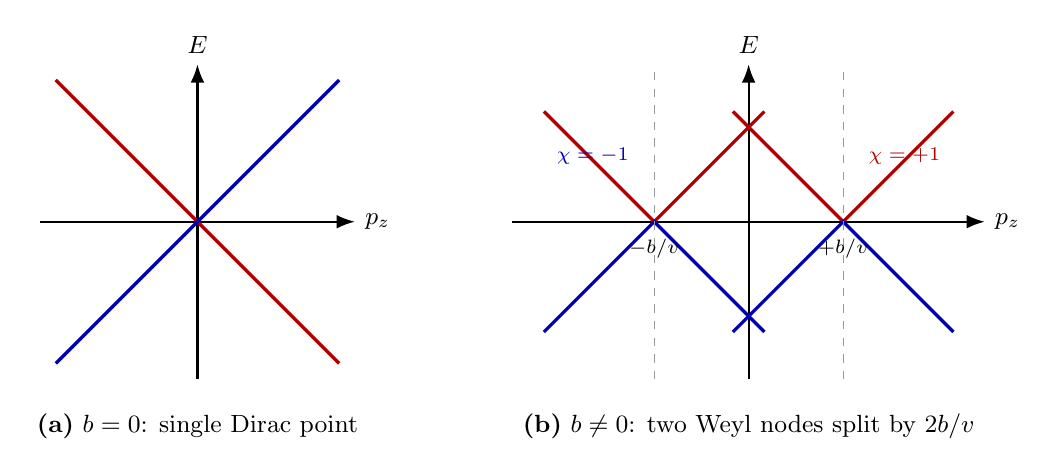
\begin{tikzpicture}[
  every node/.style={font=\small},
  axis/.style={->, >=Latex, thick},
  cone/.style={very thick},
  band/.style={very thick, color=#1},
  helpline/.style={dashed, color=black!40},
]
% --- Left: single Dirac point at p_z = 0 (b = 0)
\begin{scope}[shift={(0,0)}]
  \draw[axis] (-2,0) -- (2,0) node[right] {\(p_z\)};
  \draw[axis] (0,-2) -- (0,2) node[above] {\(E\)};
  % cone at origin
  \draw[band=red!70!black] (-1.8,1.8) -- (1.8,-1.8);
  \draw[band=blue!70!black] (-1.8,-1.8) -- (1.8,1.8);
  \node at (0,-2.6) {\textbf{(a)} $b = 0$: single Dirac point};
\end{scope}

% --- Right: two Weyl points at p_z = +/- b/v
\begin{scope}[shift={(7,0)}]
  \draw[axis] (-3,0) -- (3,0) node[right] {\(p_z\)};
  \draw[axis] (0,-2) -- (0,2) node[above] {\(E\)};
  % left Weyl node at p_z = -b/v (call it -1.2)
  \draw[band=red!70!black] (-2.6,1.4) -- (-1.2,0) -- (0.2,1.4);
  \draw[band=blue!70!black] (-2.6,-1.4) -- (-1.2,0) -- (0.2,-1.4);
  % right Weyl node at p_z = +b/v (call it 1.2)
  \draw[band=red!70!black] (-0.2,1.4) -- (1.2,0) -- (2.6,1.4);
  \draw[band=blue!70!black] (-0.2,-1.4) -- (1.2,0) -- (2.6,-1.4);
  % markers
  \draw[helpline] (-1.2,-2) -- (-1.2,2);
  \draw[helpline] (1.2,-2) -- (1.2,2);
  \node[below] at (-1.2,-0.1) {\scriptsize \(-b/v\)};
  \node[below] at (1.2,-0.1) {\scriptsize \(+b/v\)};
  \node[above right, font=\scriptsize, red!70!black] at (1.4,0.6) {\(\chi=+1\)};
  \node[above left,  font=\scriptsize, blue!70!black] at (-1.4,0.6) {\(\chi=-1\)};
  \node at (0,-2.6) {\textbf{(b)} \(b \ne 0\): two Weyl nodes split by \(2b/v\)};
\end{scope}
\end{tikzpicture}
}%
\caption{Controlled splitting of a Dirac point into two Weyl nodes by an
axial Zeeman-like perturbation $b\,\bbI\otimes\sigma_z$. The single Dirac
crossing at $\vec p = 0$ in (a) separates into two Weyl crossings of
opposite chirality along $p_z$ in (b), at $p_z = \pm b/v$.}
\label{p:fig:splitting}
\end{figure*}


\subsection{Controlled splitting Dirac \texorpdfstring{$\to$}{->} two Weyls}
A clean way to obtain a pair of Weyl nodes from a single Dirac point is
to add a Zeeman-like axial term:
\begin{equation}
\Hop \;=\; v\,\tau_{z}\otimes(\vsigma\cdot\vp)
       \;+\; b\,\bbI\otimes\sigma_{z} .
\end{equation}
Squaring gives
\begin{equation}
\Hop^{2}\;=\;(v^{2}\lvert\vp\rvert^{2} + b^{2})\,\bbI_{4}
   \;+\; 2 v b\,p_{z}\,(\tau_{z}\otimes\bbI) ,
\end{equation}
which separates as a block diagonal in $\tau_{z}$. The two blocks have
zero modes at $\vp=(0,0,\mp b/v)$ respectively, so the original Dirac
node splits into two Weyl nodes along $p_{z}$ at separation $2b/v$. The
seven Wilson-doublers analogous to the 1D case acquire masses
$m, m+2r, m+4r, m+6r$ as needed for the global lattice construction
(Sec.~\ref{p:open-problems}; \texttt{validators/desdoblamiento.py},
\texttt{validators/protoespacio\_global.py}).

\subsection{Lattice realization with Wilson term}
A concrete three-dimensional lattice realization is
\begin{equation}
\Hop(\vk) \;=\; v \sum_{i}\sin(k_{i}a)\,\alpha_{i}
       + \!\Bigl(m + r\sum_{i}\bigl(1-\cos(k_{i}a)\bigr)\Bigr)\,\beta ,
\label{p:eq:Wilson3D}
\end{equation}
with $\alpha_{i}=\tau_{x}\otimes\sigma_{i}$ and $\beta=\tau_{z}\otimes\bbI$. The
Wilson term lifts the seven naive doublers, leaving a single light Dirac
fermion at $\vk=0$. This is the lattice analogue of the structural
hierarchy in Sec.~\ref{p:setup}, and is the natural input for the
discrete data tuple of Eq.~\eqref{p:eq:proto-tuple}.


\section{Covariant structure: from \texorpdfstring{$\gamma^{\mu}$}{gamma\^mu} to \texorpdfstring{$SL(2,\mathbb{C})$}{SL(2,C)}}
\label{p:covariant}

At this point the discrete construction has reached a four-component
Dirac block whose squared dispersion is Lorentzian. The remaining task
is to identify the covariant structure that organizes it: a Clifford
algebra, the spinorial generators of Lorentz, and the connection to
$SL(2,\bbC)$.

\subsection{Clifford algebra}
In the Dirac representation, $\gamma^{0} = \tau_{z}\otimes\bbI$ and
$\gamma^{i} = \ii\,\tau_{x}\otimes\sigma_{i}$. A direct check confirms
\begin{equation}
\{\gamma^{\mu},\gamma^{\nu}\}\;=\;2\,\eta^{\mu\nu}\,\bbI_{4} ,
\qquad \eta=\mathrm{diag}(+1,-1,-1,-1) ,
\label{p:eq:clifford}
\end{equation}
which we verify entry by entry over all sixteen pairs $(\mu,\nu)$
(\texttt{validators/clifford.py}).

\subsection{Spinorial Lorentz generators}
The six spinorial Lorentz generators are
\begin{equation}
\Sigma^{\mu\nu} \;=\; \frac{\ii}{4}\,[\gamma^{\mu},\gamma^{\nu}] .
\end{equation}
Two structural facts then follow:
\begin{enumerate}[leftmargin=*]
\item the covariance identity
\begin{equation}
[\Sigma^{\rho\sigma},\,\gamma^{\mu}]
\;=\;\ii\bigl(\eta^{\sigma\mu}\gamma^{\rho}-\eta^{\rho\mu}\gamma^{\sigma}\bigr) ;
\label{p:eq:cov-id}
\end{equation}
\item the closure of the Lorentz algebra,
\begin{equation}
[\Sigma^{\mu\nu},\Sigma^{\rho\sigma}] = \ii\bigl(
  \eta^{\nu\rho}\Sigma^{\mu\sigma}-\eta^{\mu\rho}\Sigma^{\nu\sigma}
 -\eta^{\nu\sigma}\Sigma^{\mu\rho}+\eta^{\mu\sigma}\Sigma^{\nu\rho}\bigr).
\label{p:eq:lorentz-closure}
\end{equation}
\end{enumerate}
Both are verified over all 256 quadruples $(\mu,\nu,\rho,\sigma)$ by
\path{validators/lorentz.py}, covering both spinorial covariance and
Lorentz-algebra closure. Rotational generators
$\Sigma^{ij}$ are Hermitian; boost generators $\Sigma^{0i}$ are
anti-Hermitian, consistent with rotations being compact and boosts being
non-compact.

\subsection{Double cover \texorpdfstring{$SL(2,\bbC)\!\to\!SO^{+}(3,1)$}{SL(2,C) to SO+(3,1)}}
A 2$\pi$ rotation in physical space acts on a spinor as
$\mathrm{e}^{-\ii\pi\sigma_{z}} = -\bbI$, not $+\bbI$, while a 4$\pi$
rotation returns the spinor to itself. This is the standard double-cover
relation, and is verified directly by
\path{validators/puentes_grupos.py}. The chiral matrix
$\gamma_{5} = \ii\,\gamma^{0}\gamma^{1}\gamma^{2}\gamma^{3}$ anticommutes
with each $\gamma^{\mu}$ and squares to $\bbI_{4}$, defining the chiral
projectors $P_{\pm}=(\bbI\pm\gamma_{5})/2$ that decompose the four-spinor
into Weyl pairs --- closing the loop with the splitting of
Sec.~\ref{p:weyl-dirac-3d}.


\section{Emergence criteria: causality, isotropy, Nielsen--Ninomiya}
\label{p:criteria}

A consistent ladder is not enough on its own: one must also state what
counts as the relativistic limit being \emph{well posed}. We collect
three operational criteria, each verified by an explicit test.

\subsection{Effective light cone and causality}
Given a Dirac-like dispersion $E(\vp)^{2} = v^{2}\lvert\vp\rvert^{2}+m^{2}$, the
group velocity satisfies
\begin{equation}
v_{g}^{2}(\vp) - v^{2}
   \;=\; -\,\frac{m^{2}\,v^{2}}{v^{2}\lvert\vp\rvert^{2}+m^{2}} \;\le\; 0 ,
\label{p:eq:vg-bound}
\end{equation}
with saturation in the massless limit. This is the algebraic basis of
the effective light cone. The associated effective metric
\[
g^{\mu\nu}_{\mathrm{eff}}
  = \mathrm{diag}\!\left(-1,\frac{1}{v^{2}},\frac{1}{v^{2}},\frac{1}{v^{2}}\right)
\]
has the expected Lorentzian signature and determinant $-1/v^{6}$, as
checked by the causality validator. The discrete-time analogue obeys
$\cos(\varepsilon\,\Delta t) =
1-(v^{2}\vk^{2}+m^{2})\,\Delta t^{2}/2 + O(\Delta t^{3})$, recovering the
continuous dispersion at small step; see
\path{validators/causalidad_continuo_vs_discreto.py}.

\subsection{Isotropy as effective Lorentz}
For an anisotropic effective Hamiltonian
$\Hop_{\mathrm{eff}} = \sum_{a} v_{a}\,\sigma_{a}\,p_{a}$,
the squared dispersion
$\Hop_{\mathrm{eff}}^{2}=\sum_{a}v_{a}^{2}\,p_{a}^{2}\,\bbI$ reads as an
effective Riemannian metric
$g^{ab}_{\mathrm{eff}} = \mathrm{diag}(v_{x}^{2},v_{y}^{2},v_{z}^{2})$;
isotropy (a single effective light cone) is the condition
$v_{x}=v_{y}=v_{z}$. This is encoded as a SMT problem and verified by
\texttt{validators/isotropy.py}, which both confirms the existence of
isotropic solutions and the unsatisfiability of any combined
isotropy-with-anisotropy claim. For position-dependent velocities
$v_{a}(x)$ (variable tetrad) the same calculation goes through pointwise
(\texttt{validators/triada.py}).

\subsection{Chirality balance: Nielsen--Ninomiya without torus}
In the standard Nielsen--Ninomiya setting, the total chirality summed over band
nodes on a compact periodic lattice vanishes~\cite{NielsenNinomiya1981a,NielsenNinomiya1981b}. Translated to combinatorial SMT, the statement is: for
$n$ even, there exists an assignment of charges $\chi_{i}\in\{\pm 1\}$
with $\sum_{i}\chi_{i}=0$; for $n$ odd, no such assignment exists.
Moreover, no uniform-chirality configuration is allowed when the sum is
zero. This is precisely what
\texttt{validators/nielsen\_ninomiya.py} verifies.

A stronger statement holds without invoking periodicity. For a finite
bipartite graph $G=(A\sqcup B,E)$, the chirality matrix
$\Gamma=\mathrm{diag}(+\bbI_{A},-\bbI_{B})$ anticommutes with the
adjacency, and the nullity is lower-bounded by $\lvert\lvert A\rvert-\lvert B\rvert\rvert$. On
a maximum matching the bound saturates. These facts, contained in
\texttt{validators/rama\_estructural.py}, are exactly the discrete index
theorem in the absence of reciprocal-space periodicity --- a key
ingredient of the structural branch of Sec.~\ref{p:open-problems}.

\subsection{Wilson term and the selection of the light Dirac}
On the 3D Wilson--Dirac lattice of Eq.~\eqref{p:eq:Wilson3D}, the
seven Brillouin-zone corners other than $\vk=0$ acquire Wilson masses
$m+2r, m+4r, m+6r$ depending on their distance from the origin in $\pi/a$
units, while $\vk=0$ retains mass $m$. This is the Wilson lattice mechanism~\cite{Wilson1974}
that lifts the naive fermion doublers and isolates a single light Dirac
in the infrared (\texttt{validators/wilson\_subsector.py},
\texttt{validators/protoespacio\_global.py}).


\section{Verification methodology}
\label{p:verification}

The verification policy underlying the paper is simple to state and deliberately limited in scope: the algebraic and finite combinatorial claims that support the infrared construction are paired with executable tests. The tests do not certify the full analytic continuum limit, but they do make the matrix identities, expansions, and finite obstruction statements auditable.

\paragraph{Two backends, one policy.}
Algebraic identities are checked by \texttt{sympy}, which is appropriate when the claim is an equality between matrix expressions, an expansion to first or second order, or a manipulation of Clifford or Pauli algebra. Combinatorial and order-theoretic claims (Nielsen--Ninomiya balance, isotropy as SMT, bipartite index, structural consistency of small causal sets) are checked by the SMT solver \texttt{z3}~\cite{deMoura2008}, which is appropriate when the natural domain is propositional or arithmetic over small finite types.

\paragraph{Granularity.}
Each claim intended to be mechanically checked is linked to a validator by a comment of the form
\begin{center}\small\texttt{\% verified-by: validators/\textless module\textgreater.py::\textless test\textgreater}\end{center}
placed near the corresponding derivation. This makes the manuscript navigable at the claim level: the reader can move from an equation to the specific test that checks it.

\paragraph{Pipeline.}
A build script runs the test suite through \texttt{pytest} and proceeds with \texttt{latexmk} only on a clean exit. In the current development tree, the suite contains $146$ tests and runs in under twenty seconds on a standard laptop. Of particular note: the policy caught three classes of errors during development. (i) An overconfident formulation of a chirality predicate based on the wrong combinatorial restriction, which the SMT failed correctly. (ii) A wrong sign in the spinorial covariance identity Eq.~\eqref{p:eq:cov-id}, caught by the closed-form symbolic test. (iii) An inversion of the Hermitian / anti-Hermitian status of rotational vs. boost generators in docstrings, detected by \texttt{::test\_rotation\_generators\_hermitian} and \texttt{::test\_boost\_generators\_antihermitian}. In each case the correction was algorithmic, not interpretive.

\paragraph{Cost / benefit.}
The cost of writing a verification module per claim is approximately two to four hours of careful work; the cost of running the full suite is negligible. The benefit is more important: the manuscript becomes \emph{auditable}. A reader who wants to confirm a specific algebraic identity can inspect the corresponding test without needing to rerun the full derivation by hand.

\paragraph{Comparison with proof assistants.}
The present approach is deliberately coarser than a Lean/Coq/Isabelle formalization. \texttt{sympy} and \texttt{z3} suffice for the algebraic and combinatorial layer certified here, do not require re-encoding the entire physics in a typed proof assistant, and integrate naturally with a conventional theoretical-physics workflow. The trade-off is that we certify local algebraic facts, not all functional-analytic assumptions behind the continuum limit. That limitation is explicit.


\section{Open structural problems}
\label{p:open-problems}

The verified infrared ladder narrows the remaining problem. Once Dirac covariance has been recovered as an infrared organization, the next question is not whether the Dirac algebra can appear, but what microscopic data are sufficient for such a sector without relying on Bloch periodicity as the primary language. We separate this into a spectral branch and a structural branch.

\subsection{Spectral branch: global classification on the Brillouin torus}
The local infrared analysis of band crossings says little about the \emph{global} structure of the discrete quasi-energy. Two facts have been verified: the quasi-energy is circular ($\varepsilon\in[-\pi,\pi]$ in units of $\Delta t$), and the two sectors $\omega=0$ and $\omega=\pi$ can both host band-crossing points. For the canonical 1D walk $\Uop(k) = \cos(k)\bbI - \ii\sin(k)\sigma_{z}$ a direct check confirms that $\Uop(0)=\bbI$ and $\Uop(\pi)=-\bbI$, placing band touchings at both $\omega=0$ and $\omega=\pi$. In three dimensions the corner family of the cubic Brillouin zone admits an assignment of $\chi=\pm 1$ to its eight vertices with total sum zero and a 4-and-4 distribution between the two quasi-energy sectors --- a satisfiable SMT problem when stated correctly, and unsatisfiable when one demands an imbalance such as $5$ vs. $3$ (\texttt{validators/brillouin\_global.py}).

The open question is a \emph{complete} classification of special points of the spectrum of $\Uop(\vk)$ over the 3D Brillouin zone, taking into account the exact symmetries of the discrete step. The present verification machinery covers the local algebra and the corner combinatorics; what remains is the cohomological/global part of the picture.

\subsection{Structural branch: protospace without reciprocal language}
The deeper open question is whether the underlying $\Proto$ admits a formulation that does not assume a torus or reciprocal-space description to begin with. Three concrete sub-tasks are already sharply formulated:

\begin{itemize}[leftmargin=*]
\item \textbf{(E1) Local discrete data beyond periodic lattices.} Formulate $\Proto = (\Lattice,\bbC^{N},\Uop,G_{\mathrm{micro}})$ on local graphs not assumed to be periodic. Verified examples include a tight-binding Hamiltonian on a chain of $n$ sites and on a deliberately irregular graph of 6 sites with mixed vertex degrees, where $\Uop_{\Delta t} = \bbI - \ii\Delta t\,\Hop + O(\Delta t^{2})$ has the nearest-neighbour support pattern dictated by the graph adjacency.
\item \textbf{(E2) Infrared stability without exact translation.} Test whether effective Dirac sectors survive perturbations that break exact translation while preserving locality. Verified examples include bond-disordered SSH Hamiltonians for which the discrete chiral symmetry $\Gamma$ anticommutes with $\Hop$, forcing the spectrum to remain $\{-E,E\}$-symmetric without Fourier analysis.
\item \textbf{(E3) Chirality balance without a Bloch torus.} Formulate a combinatorial replacement for chiral balance on finite graphs. Verified: for a bipartite graph $G=(A\sqcup B,E)$ the nullity of the adjacency is lower-bounded by $\lvert\lvert A\rvert-\lvert B\rvert\rvert$, the discrete index. On a maximum matching the bound saturates exactly.
\end{itemize}

These structural problems are open but well posed: the algebra and finite combinatorics required to formulate them on arbitrary graphs are already executable; what is missing is a selection principle that identifies which local graph/step structures deserve to count as admissible protospaces.


\section{Conclusions}
\label{p:conclusions}

We have constructed a discrete-to-continuous ladder
\[
\text{SSH} \to \text{graphene} \to \text{honeycomb QW} \to \text{Weyl/Dirac 3+1}
\]
with uniform notation, three explicitly separated levels, and a verification discipline that pairs the algebraic and finite combinatorial claims with symbolic tests.

The relativistic structure --- the Clifford algebra of $\gamma^{\mu}$, the spinorial Lorentz generators $\Sigma^{\mu\nu}$, the double cover by $SL(2,\bbC)$, an effective Lorentzian light cone with controlled group velocity, and chirality balance constraints --- appears as an infrared organization of local discrete dynamics, not as an exact microscopic symmetry of the step.

The verification methodology is the most reusable part of the construction. It does not require interactive theorem provers, integrates with the working scientist's existing toolchain, and yields manuscripts whose algebraic claims are locally auditable. The resulting standard is modest but useful: do not merely state the identity that supports an infrared limit; make the identity executable.

The construction also sharpens the next problem. Once the infrared Dirac ladder is under control, the deeper structural question becomes how to formulate locality, chirality, and Dirac sectors without taking reciprocal-space periodicity as fundamental. In that sense, the present paper turns the problem of protospace into a more precise question: not whether Dirac covariance can emerge in the infrared, but what microscopic data are sufficient for such an infrared sector to exist.

\section*{Acknowledgements}
The author thanks the open-source scientific Python and TeX communities whose tools made the verification and typesetting workflow possible. AI-assisted coding and editorial tools were used to help draft, refactor, and review parts of the validation modules, tests, and manuscript text; all scientific claims, validator design choices, and final interpretations remain the responsibility of the author.

\section*{Data and code availability}
The validators referenced throughout the manuscript are maintained in the companion project repository at \url{https://github.com/xys004/protoespacio-validation}. A public archival DOI should be inserted here before journal submission if a frozen release is deposited.


\begin{thebibliography}{99}

\bibitem{Su1979}
W.~P. Su, J.~R. Schrieffer, and A.~J. Heeger,
Solitons in polyacetylene,
\emph{Physical Review Letters} \textbf{42}, 1698--1701 (1979).
\href{https://doi.org/10.1103/PhysRevLett.42.1698}{doi:10.1103/PhysRevLett.42.1698}.

\bibitem{Wilson1974}
K.~G. Wilson,
Confinement of quarks,
\emph{Physical Review D} \textbf{10}, 2445--2459 (1974).
\href{https://doi.org/10.1103/PhysRevD.10.2445}{doi:10.1103/PhysRevD.10.2445}.

\bibitem{NielsenNinomiya1981a}
H.~B. Nielsen and M.~Ninomiya,
Absence of neutrinos on a lattice. I. Proof by homotopy theory,
\emph{Nuclear Physics B} \textbf{185}, 20--40 (1981).
\href{https://doi.org/10.1016/0550-3213(81)90361-8}{doi:10.1016/0550-3213(81)90361-8}.

\bibitem{NielsenNinomiya1981b}
H.~B. Nielsen and M.~Ninomiya,
Absence of neutrinos on a lattice. II. Intuitive topological proof,
\emph{Nuclear Physics B} \textbf{193}, 173--194 (1981).
\href{https://doi.org/10.1016/0550-3213(81)90524-1}{doi:10.1016/0550-3213(81)90524-1}.

\bibitem{Semenoff1984}
G.~W. Semenoff,
Condensed-matter simulation of a three-dimensional anomaly,
\emph{Physical Review Letters} \textbf{53}, 2449--2452 (1984).
\href{https://doi.org/10.1103/PhysRevLett.53.2449}{doi:10.1103/PhysRevLett.53.2449}.

\bibitem{CastroNeto2009}
A.~H. Castro Neto, F.~Guinea, N.~M.~R. Peres, K.~S. Novoselov, and A.~K. Geim,
The electronic properties of graphene,
\emph{Reviews of Modern Physics} \textbf{81}, 109--162 (2009).
\href{https://doi.org/10.1103/RevModPhys.81.109}{doi:10.1103/RevModPhys.81.109}.

\bibitem{Arrighi2018}
P.~Arrighi, G.~Di~Molfetta, I.~M\'arquez-Mart\'in, and A.~P\'erez,
The Dirac equation as a quantum walk over the honeycomb and triangular lattices,
\emph{Physical Review A} \textbf{97}, 062111 (2018).
\href{https://doi.org/10.1103/PhysRevA.97.062111}{doi:10.1103/PhysRevA.97.062111}.

\bibitem{FarrellyShort2014}
T.~C. Farrelly and A.~J. Short,
Causal fermions in discrete space-time,
\emph{Physical Review A} \textbf{89}, 012302 (2014).
\href{https://doi.org/10.1103/PhysRevA.89.012302}{doi:10.1103/PhysRevA.89.012302}.

\bibitem{Farrelly2020}
T.~C. Farrelly,
A review of quantum cellular automata,
\emph{Quantum} \textbf{4}, 368 (2020).
\href{https://doi.org/10.22331/q-2020-11-30-368}{doi:10.22331/q-2020-11-30-368}.

\bibitem{deMoura2008}
L.~de Moura and N.~Bj{\o}rner,
Z3: An efficient SMT solver,
in \emph{Tools and Algorithms for the Construction and Analysis of Systems},
Lecture Notes in Computer Science \textbf{4963}, 337--340 (Springer, 2008).
\href{https://doi.org/10.1007/978-3-540-78800-3_24}{doi:10.1007/978-3-540-78800-3\_24}.

\end{thebibliography}



\end{document}
